\chapter{Team 6 Agent Design}
\section{Introduction} \label{sec:Team6_Intro}
Our agent/island, which is on behalf of one of the islands sitting on the archipelago, has some basic properties controlling the overall behaviour. Three main properties includes \emph{Personality}, \emph{Friendship} and \emph{Trust Rank}. \emph{Personality} implicitly refers to the amount of the resources our island currently holds. There are three tiers of personality, each makes our island perform different actions during the interaction with other islands. The more resources we have, the more generous our island is. \emph{Friendship} is a map containing keys as islands and values as the friendliness with certain island. It measures the relationship between our islands and the others, and can be either increased or decreased. The changes happens mostly at the IITO session of each turn, when the gifts are exchanged. For example, if the total amount of gifts we have received from an island is less than the amount of gifts we sent to an island, the friendship level with that island will be reduced by how much the difference between our gifts. \emph{Trust Rank} determines how much our island can trust an island. It is then used to Judge the way we consider their prediction of a disaster in the IIFO session. For islands holding less trust rank with us, their prediction results will be applied with a weight factor that heavily penalises the result. The final prediction for IIFO is the mean value of the predictions from all 6 islands.

\section{Design and Implementation} \label{sec:Team6_design_impl}

\subsection{IIGO} \label{subsec:Team6_IIGO}
In IIGO session, besides the collaboration of three distinct branches to maintain, update and revise the rule, decision regarding allocation request from common pool is made by each agent. Agents are required to act in this session based on their resources availability. The decision-making actions which are required from each island are:
\begin{itemize}
    \item contribute resources to the common pool in form of taxation which is the minimum amount set by the President.
    \item request resources from the common pool.
    \item vote in favor/against the proposed rule made by the President.
    \item vote in the election of Judge, Speaker, and President.
\end{itemize}
There are two potential problems that could arise in this situation:
\begin{itemize}
\item an agent can request resources much more than necessary. As a result, there are not enough resources in Common Pool for other agents to request, i.e., agents lose the opportunity to generate resources and have less ability to participate in foraging. Therefore, agents will get less return from foraging. This problem follows the notion of micro-level goal, which states that a self-interested agent will try to satisfy maximally; and also the concept of the tragedy of the common proposed by Gerit Hardin, which says that people will make a decision that maximises their interests in the short term, even if this leads to the deterioration of the common pool resource in the long run, which is in nobody's interest~\footnote{Pitt, J. \textit{Self-Organising Multi-Agent Systems} (p. 156). IC Press.}.
    \item an agent requests too few of resources, as there are not sufficient resources in the Common Pool. This also has a negative effect on agent’s ability to invest in foraging. Consequently, the agent will less likely to survive. 
\end{itemize}

\subsubsection{Strategies} \label{subsubsec:Team6_IIGO:Strategies}
Our agent has the personality which is based on the current amount of resources. The personality parameter is a dynamic variable that is adjustable, and helps assisting agent’s decision in any event related to economic aspect. These personalities consist of normal, selfish, and generous. This parameter is used to determine whether or not we would like to request resources from the common pool. 

\subsubsection{Implementation} \label{subsubsec:Team6_IIGO:Implementation}
\begin{itemize}
\item \textbf{Request Allocation}: when the current resource is below the minimum threshold, the difference of minimum threshold minus current resource will be requested. If the current resource is above threshold, the request will depend on the personality. If the allocation amount determined is not enough for living cost and the current personality is selfish, the agent will take the amount equals to living cost. In other situations, only the resources allocated will be taken.
\item \textbf{Common Pool Resource Request}: when our island is not in critical status and the current resource is larger than the minimum threshold, the common pool resource will be requested based on the personality. In generous mode, our agent will only ask for living cost of one day, otherwise we will ask for three times of the living cost. However, more resources allocated means more contribution in foraging and can bring abundant return and subsequently abundant tax will be paid after.
\item \textbf{Tax Contribution}: in normal situation, the exact tax amount determined by the President will be paid. However, no tax will be paid if we are in critical status. When the disaster is approaching (our prediction for the time left $< 1$) and the current personality is generous, more tax will be paid. 
\item \textbf {Sanction Payment}: sanction will be paid if our island is not in critical status. If our resource can be lower than the minimum threshold after paying the determined sanction amount, then we will try to only pay partially above the threshold. 
\item \textbf {Resource report}: when the personality of the agent is selfish, only a half of the actual resource will be reported in order to get more allocation.
\end{itemize}
%\subsubsection{Opinions}

\subsection{IITO} \label{subsec:Team6_IITO}
\subsubsection{Trust and Relationship Dilemma} \label{subsubsec:Team6_IITO:Dilemma}
In IITO sessions, communications and interactions among the islands/agents happen during the game to exchange information, besides governance-related information which happens in IIGO sessions, with details mentioned in Subsection~\ref{subsec:IITO:inter_island_communication}. The highlight for agent strategy in IITO sessions is especially related to the actions of giving and receiving gifts to/from other island(s) in terms of resources. Islands are required to act in this session based on the resource information of their own private pool and/or of other island's if available (i.e. islands are willing to share resource information to other islands).

As described in Subsection~\ref{subsec:IITO:gifting_session}, the decision-making actions that are required from the island are, whether the island wishes to:
\begin{itemize}
    \item request gifts of certain amount of resources from specific island(s).
    \item offer gifts of certain amount of resources to specific island(s).
    \item respond to gifts of certain amount of resources offered to them from the other island(s), provided some available choices i.e. to accept the full amount of the offered gifts, to accept partial amount of the offered gifts, or to decline the offered gifts.
    \item update the history of the above three events (including the amount) to be informed to the respective island(s).
\end{itemize}

The potential emerging dilemma in this part is related to decision-making under uncertainty from social construction of the agents' social interaction. In this context, the concept of \emph{trust} is introduced as a key factor in the social relations. According to the trust framework~\footnote{Pitt, J. \textit{Self-Organising Multi-Agent Systems} (pp. 234-235). IC Press.}, there are three aspects that affect the perspective of one's decision-making in social relations:
\begin{itemize}
    \item cognitive dimension: beliefs, interpretation of signals, etc.
    \item economic dimension: utility, cost/benefit analysis, etc.
    \item normative dimension: rule, expectation of conformance or punishment for non-compliance, etc.
\end{itemize}
We mainly focus on the economic dimension as it is the measurable parameter in the game that is helpful for the decision-making.

\subsubsection{Strategies} \label{subsubsec:Team6_IITO:Strategies}
Based on the economic dimension for decision-making as mentioned in the above, our agent strategy for taking actions on this gifting mechanism is parameterised by the following aspects:
\begin{itemize}
    \item current status of our island and other islands at current state of the game, i.e. alive, critical or dead, including the counter of the critical status (how many turns stay in critical status).
    \item chosen personality mode of our island at current state of the game, i.e. selfish, normal or generous.
    \item current resource level in our island's private pool with some considered factors such as a minimum threshold for disaster coverage, and the cost of living.
    \item level of friendship between our island and the other island(s) correspondingly by using friendship coefficient.
\end{itemize}
For requesting gifts from other island(s), firstly we do not request for any gift from the island(s) that is/are not alive at the state of the game. Then, in order to survive the game, our island submit the request to all islands if we are in critical status (current resource level is less than the minimum threshold) with the value requested is the amount of minimum threshold. Otherwise, if our island is not in critical status, we would still submit request for gifts to other islands, but it depends on the personality mode we are playing at the state of the game that proportional to a multiplier factor (\emph{friendship coefficient}) to the value of cost of living.

For offering gifts to other island(s), firstly we do not offer any gift to any other islands if we are in the critical status at the state of the game, as this is part of the self-preservation mechanism of our own resource level to survive. Secondly, we prioritise the other islands who are in critical status, thus we offer them a minimum threshold value of resources to help them survived, as part of the common goal for sustainability of the archipelago. Otherwise, for non-critical circumstances, the strategies depend on the friendship level and the chosen personality of our own island. Friendship level sorts out on the preference which island we offer the gift to with the proportion amount of resources that do not make our island goes to critical level. Meanwhile, the chosen personality of our island introduces a penalty factor to the gift offers we received by using the friendship coefficient. When we are generous, no penalty is used, thus our island accept the received offers given to us.

For gifts responses, firstly we just accept all gifts of the offered amount of resources from any island if we are in the critical status. Otherwise, we also just decline the offered gifts from islands that are in critical status to save their resources. Under normal circumstances, our island responds to the gifts from other islands based on the friendship level, i.e. decline it when the island has minimum level of friendship with our island, or accept it partially (with the deduction of cost of living) when the island has maximum level of friendship with us.

\subsubsection{Implementation} \label{subsubsec:Team6_IITO:Implementation}
The gift exchanging is the main activity during the IITO session where each island exchanges some of their resources, known as \emph{gift}, with the other islands. The behaviour of our island for gifting will be controlled by two of our main properties: \emph{Friendship} and \emph{Personality}. In general, the less resources we have in our private pool, the more egocentric our island will be. Nevertheless, in each turn of the IITO session, there are some extra checking to be done before performing our specific behaviour based on these properties. Firstly, if we find our island is in the critical status, which means we are going to die in a few turns to come, we will instantly decide that there will be no gift to be sent to anyone in this round. Otherwise, there will be gifts from us sent to other islands. The islands in critical status hold the privilege to certainly receive a few amount of gifts from us in order to help them out of the critical status, as we bear in mind the fact that the maximum chance of survival of any single island depends on the survival of all islands. After checking these priorities, we then determine what gifts we send to the other islands in non-critical status.
\begin{algorithm}[H]
\SetAlgoLined
    \uIf{Personality == Selfish}{
        request gifts scaled up by friendship coefficients\;
    }
    \uElseIf{Personality == Normal}{
        request gifts without scaling\;
    }
    \uElseIf{Personality == Generous}{
        request gifts scaled down by friendship coefficients\;
    }
    \caption{Gifts Requests}
\end{algorithm}

\begin{algorithm}[H]
\SetAlgoLined
    \uIf{Personality == Selfish}{
        request gifts scaled down by friendship coefficients\;
    }
    \uElseIf{Personality == Normal}{
        request gifts without scaling\;
    }
    \uElseIf{Personality == Generous}{
        request gifts scaled up by friendship coefficients\;
    }
    \caption{Gifts Offers}
\end{algorithm}


The algorithm above concludes how our agent makes use of Friendship and Personality, and behaves differently during the gift exchanging section. Basically, the amount of any gifts can be linearly scaled based on how much friendship we have with the target island whom we are requesting or offering gifts to. For example, if our island is \emph{selfish}, the amount of the gift we offer will be scaled down by a value depending on the current friendship. A relative coefficient will be calculated based on that. If the island is a good friend with us, the coefficient will be relatively lower when it comes to the gift offers, so that the amount by which it is scaled down will be less. Otherwise, the coefficient will be higher and a higher penalty will be applied so that we offer our bad friend very few gifts.
%\subsubsection{Opinions}

\subsection{IIFO} \label{subsec:Team6_IIFO}
\subsubsection{Long-Term Collective Risk Dilemma} \label{subsubsec:Team6_IIFO:ltCRD}
% Individual utilities vs CPR
Our agent faces a cost of living deducted at every turn, and an expenditure when a disaster hits. To mitigate the effect of disaster, islands make contributions to the common-pool. The long-term collective risk dilemma (ltCRD) defines that how much resources are needed to be raised and before when. We parameterise such problem with a threshold $T$ and a deadline day $D$.


\subsubsection{Strategies} \label{subsubsec:Team6_IIFO:Strategies}
In this coursework, there are non-stochastic and stochastic disasters. For the non-stochastic disaster, $T$ is known and $D$ is unknown. For the stochastic disaster, both $T$ and $D$ are unknown. To deal with ltCRD, the islands make forecast about $T$ and $D$, whereas each island has its own knowledge to predict the disaster. On the one hand, when an individual island forms an opinion regarding the desired contribution to the common-pool resources, it is necessary to convince others that the decision is rational. On the other hand, we take the aggregate knowledge into consideration, taking advantages of distributed computation of disaster prediction. Such prediction information comprises:
\begin{itemize}
    \item the coordinates.
    \item the magnitude of disasters.
    \item the confidence of prediction.
\end{itemize}
The recommendation of common-pool resource contribution is based on the comparison among our own prediction and shared predictions from others. 

\subsubsection{Implementation} \label{subsubsec:Team6_IIFO:Implementation}
For the foraging, islands can share the most recent foraging decisions they made and the resources obtained to other islands. There is a \texttt{ShareTo} list containing island IDs that our island wishes to share this information with. The following pseudocode describes the logic in our disaster prediction:
\begin{algorithm}[H]
\SetAlgoLined
    \uIf{not knowing the period \textbf{and} not knowing whether it's stochastic}{
        check the disaster history\;
        find if it is stochastic\;
        find the disaster period\;
    }
    \uElseIf{knowing the period \textbf{and} not knowing whether it's stochastic}{
        check the disaster history\;
        find if it is stochastic\;
    }
    \uElseIf{not knowing the period \textbf{and} knowing whether it's stochastic}{
        check the disaster history\;
        find the disaster period\;
    }
    decide the prediction based on the period and stochastic information we have\;
    \caption{Disaster Prediction}
\end{algorithm}


Since the coordinates of a happening disaster follows a uniform distribution which makes it totally random and unpredictable, our island focuses the prediction on the time left for a disaster to happen in different ways based on whether or not the settings of period and stochastic disaster is exposed. It is possible to calculate the exact time of a disaster if it is not stochastic. Otherwise, the possibility of a disaster can be calculated based on the period if it is stochastic. For either case, it is assumed that the period and the stochastic condition are exposed to our agent. However, chances are that one or both of these settings are not exposed to us. In this case, our agent will look through our disaster history and try to find the settings based on the patterns. For example, if the agent finds the time period between any two disasters is not identical, then it will reckon the disaster period to be stochastic. Otherwise, if it find all the period between any of the two disaster is the same, the agent will consider the setting of disaster is not stochastic, where there is a fixed period between the disasters. Based on the final prediction we have made, our island will determine how much resources we want to invest to the common pool to mitigate the disaster impact.

%\subsubsection{Opinions}

\subsection{Foraging} \label{subsec:Team6_Foraging}
\subsubsection{Risk-Payoff Dilemma} \label{subsubsec:Team6_Foraging:RP_dilemma}
In each turn, our agent has an opportunity to gain resources from the environment by foraging. Such action can be regarded as an investment of resources by deciding:
\begin{itemize}
    \item the type of foraging i.e. either deer hunting or fishing.
    \item the quantity of resources that our agent invests.
\end{itemize}
The consideration of risk and payoff underpins the rationale of decision-making. Within the context of this coursework, deer hunting offers a high amount of payoff with high risk, whereas fishing is a low-risk decision with relatively lower returns. The dilemma of risk and payoff has been studied in Stag Hunt Game~\footnote{Pitt, J. \textit{Self-Organising Multi-Agent Systems} (pp. 84-85). IC Press.}, where the difference of outcome between the safe option and the risky option affects the preferable choice. By introducing return on investment (ROI) regarding the total investments on deer hunting and fishing, our agent can estimate the difference between safe and risky investments.

\subsubsection{Inter-Foraging-Group Dilemma} \label{subsubsec:Team6_Foraging:Group_dilemma}

According to Kitchen Stand-Off game~\footnote{Pitt, J. \textit{Self-Organising Multi-Agent Systems} (pp. 67-68). IC Press.}, social welfare can be maintained by not necessarily the cooperation, while a huge individual contribution can unilaterally support it. In this coursework, the quantity of investments from individual agents foraging together determines the level of return. In fishing, the return to all participants is equally distributed as long as the total investment reaches a certain value. This brings out the dilemma between individual contribution and collective return. 

Table~\ref{table:FishAbundant} and~\ref{table:FishScarce} presents the possible outcomes introduced by the decision on fishing. 

\begin{table}[!htb]
    \setlength{\extrarowheight}{2pt}
    %\centering
    \begin{tabular}{cc|c|c|}
      & \multicolumn{1}{c}{} & \multicolumn{2}{c}{Other Agents' Total Investment}\\
      & \multicolumn{1}{c}{} & \multicolumn{1}{c}{$Low$}  & \multicolumn{1}{c}{$High$} \\\cline{3-4}
      \multirow{2}*{Our Agent's Investment}  & $Low$ & $(1,1)$ & $(2,4)$ \\\cline{3-4}
      & $High$ & $(4,2)$ & $(3,3)$ \\\cline{3-4}
    \end{tabular}
    \caption{Decision Matrix - When the population of fish is abundant.}\label{table:FishAbundant}
\end{table}

\begin{table}[!htb]
    \setlength{\extrarowheight}{2pt}
    %\centering
    \begin{tabular}{cc|c|c|}
      & \multicolumn{1}{c}{} & \multicolumn{2}{c}{Other Agents' Total Investment}\\
      & \multicolumn{1}{c}{} & \multicolumn{1}{c}{$Low$}  & \multicolumn{1}{c}{$High$} \\\cline{3-4}
      \multirow{2}*{Our Agent's Investment}  & $Low$ & $(1,1)$ & $(0,2)$ \\\cline{3-4}
      & $High$ & $(2,0)$ & $(0,0)$ \\\cline{3-4}
    \end{tabular}
    \caption{Decision Matrix - When the population of fish is scarce.}\label{table:FishScarce}
\end{table}
\subsubsection{Strategies} \label{subsubsec:Team6_Foraging:Strategies}
Backtracking foraging history allows us to monitor the trend of ROI and capital input. The qualitative opinion formation is based on historical foraging information exchanged in IIFO session: 
\begin{itemize}
    \item overall resource input to foraging increases, which indicates that the high-tier foraging return is likely to obtained. In such case, increasing our input is preferred.
    \item overall resource input to foraging decreases, which indicates that the low-tier foraging return is likely to obtained. In such case, reducing our input is preferred.
\end{itemize}

The quantitative decision regarding the amount of investment refers to the amount that we invested in previous turns. Such amount of extra input or less input is determined by our current personality. Referring to the decision matrix~\ref{table:FishAbundant} and~\ref{table:FishScarce}, we gain more benefits when the overall investment is high and our investment is lower than others. This implies a high efficiency of foraging from our perspective. However, if the gap between the average of total investments and ours is large enough, it will not be sustainable for other islands due to their relatively lower foraging efficiencies. Hence, we follow:
\begin{itemize}
    \item when the overall resource input to foraging increases, we increase the investment but not higher than the average of investment, which is estimated by historical overall investments.
    \item when the overall resource input to foraging decreases, we decrease the investment or consider changing the foraging type.
\end{itemize}


\subsubsection{Implementation} \label{subsubsec:Team6_Foraging:Implementation}
There is a map that records all the forging history. Our agent will do two deer hunting and one fish hunting at the first three rounds, as there are insufficient items in the map for running the algorithm. Contribution to the foraging is calculated by using a multiplier for the value of current amount of our resources minus safety buffer. The safety buffer is calculated by adding the Cost of Living and the Minimum Resource Threshold, which are determined in the server. The multiplier is adjusted by analysing the ROI (Return on Investment) trending. The multiplier will be larger if the trending is increasing, and will be smaller otherwise.

The forging type for current turn is decided by comparing the average ROI of total deer hunting with the total fishing from the last turn. The one with better average ROI will be chosen.

\begin{algorithm}[H]
\caption{Foraging} 
    %\begin{algorithmc}
    calculate the average ROI for deer hunting last turn $\alpha_1$\;
    calculate the average ROI for fish hunting last turn  $\beta_1$\;
    calculate the average ROI for deer hunting 2 rounds before $\alpha_2$\;
    calculate the average ROI for fish hunting 2 rounds before $\beta_2$\;
    \If{$\alpha_1 > \beta_1$}{
        \If{$\alpha_1 > \alpha_2$}{$multiplier \gets multiplier + 0.05$\;}
        \Else{$multiplier \gets multiplier - 0.05$\;}
        \Return deer type\;
    }
    \Else{
        \If{$\beta_1 > \beta_2$}{$multiplier \gets multiplier + 0.03$\;}
        \Else{$multiplier \gets multiplier - 0.03$\;}
        \Return fish type\;
    }
    %\end{algorithmc}
\end{algorithm}

Since fishing is a safer choice than deer hunting, the sumand used in deer hunting will be larger than that in fishing. The general idea for this algorithm is to calculate the differential of the total ROI history curve. Due to time limit, the difference value between the last round and 2 rounds before is used to replace the differential.

\subsection{President} \label{subsec:Team6_President}
\subsubsection{Individual taxation problem} \label{subsubsec:Team6_President:Dilemma}
In each turn, the President has the power to decide the taxation amount which is a minimum amount of contribution to the common pool for each island. The President is given a self-reported amount from each island to help assist President’s decision. The taxation is directly related to the common pool resource, so the President has a huge impact on the sustainability of the common pool. In fact, in our coursework, some conditions of zero contribution thesis proposed by Mancur Olson are already met~\footnote{Pitt, J. \textit{Self-Organising Multi-Agent Systems} (p. 160). IC Press.}. There is some form of coercion which is a taxation in our case. Thus, It is safe to say that the sustainability of the common pool resource is possible.

However, a problem could emerge when deciding the appropriate amount of taxation. The common criteria the President use to evaluate the taxation is the available amount of resource for each island. For example, the President could set taxation amount by using some fixed tax rate which will be multiplied by reported amount of resource for each island. It is not a trivial task to decide the most appropriate taxation amount because numerous factors should be considered before the decision could be made, and each island also gets different level of severity based on the disaster’s location and damage. The major drawback from this fixed tax rate approach is that it does not take into account the overall behaviour of each islands, which could greatly differ from island to island. In this context, the notion of Distributive Justice is introduced as one of fundamental factors in the analysis of social interaction.

\subsubsection{Strategies} \label{subsubsec:Team6_President:Strategies}
For our agent strategy, inspired by Distributive Justice theories, namely equity and need~\footnote{Pitt, J. \textit{Self-Organising Multi-Agent Systems} (p. 195). IC Press.}, which concerns about the welfare of least advantaged agents, the status of individual islands should be one of main parameters that can be used to determine the current status of islands, i.e. the taxation amount will be proportional to the degree of severity the island has. The status of the island is affected by several variables and events in the game such as the damage from disaster or the current amount of resource. Therefore, the status parameter is utilised to decide to most appropriate taxation amount. Additionally, the second strategy used in our agent is based on the concept of friendship for decision making. Taxation amount can be determined by friendship coefficient. The coefficient is based on the level of friendship between our agent and other agents. For instance, if an island has a maximum level of friendship, there will be no taxation for that island. But if the level of friendship is very low, our agent will set a tax rate which will be multiplied by friendship coefficient. The friendship system is related to each island’s overall behaviours which affect our agent throughout the game. A well-behaved island deserves lower amount of taxation, and vice versa. 

\subsubsection{Implementation} \label{subsubsec:Team6_President:Implementation}
The implementation basically follows the base implementation which is pre-defined in the IIGO section. Additionally, our island is possible to be an unreasonable President if we are holding a few amount of resources, which is then measured by our personality.

For this implementation, our agent utilises the personality property in addition to the evaluation as a President of all other islands. When our island is selfish, we will try to take advantage of our privilege as a President and try to allocate the resources we have requested from the common pool first, so that we have the highest chance to successfully acquire the allocated resources.

\begin{algorithm}[H]
\SetAlgoLined
    \uIf{Personality != Selfish}{
        \uIf{resources requested < available common pool}{
            distribute the allocation for all islands\;
        }
        \Else
        {
            distribute a portion of the allocation for all islands\;
        }
    }
    \Else{
        \uIf{resources requested from us < available common pool}{
            distribute the allocation for us\;
        }
        \Else{
            distribute a portion of the allocation for us\;
        }
        \uIf{resources requested from other islands < common pool left}{
            distribute the allocation for other islands\;
        }
        \Else{
            distribute a portion of the allocation for other islands\;
        }
    }
    \caption{Evaluating the allocation request}
\end{algorithm}

\subsubsection{Opinion} \label{subsubsec:Team6_President:Opinion}
In our game implementation, the fact that President is able to freely choose tax rate is not beneficial to islands’ survivability. This rate should be dynamic and adjustable according to islands’ available resources and several other factors such as overall behaviour and their history of contribution to the common pool, which is not implemented in our game. In our opinion, these drawbacks can be mitigated by introducing reliable parameters which reflect islands’ overall performance and responsibility.

\subsection{Speaker} \label{subsec:Team6_Speaker}
\subsubsection{Monitoring Problem} \label{subsubsec:Team6_Speaker:Problem}
In each turn, Speaker has the power to call a vote for a rule and also the election of roles, decide the voting result, and whether to broadcast this information to other islands. Vote from each island is given to Speaker and the result can be made.
A potential problem could arise when it comes to declaring the result, i.e. Speaker can cheat and make false information regarding the voting result. In our coursework, the accountability cycle has been introduced to handle and monitor this potential abuse of power. However, this monitoring power is of one degree. In other words, the power pertaining to the accountability cycle will not be monitored themselves. This calls for an alternative solution.

\subsubsection{Strategies} \label{subsubsec:Team6_Speaker:Strategies}
Our agent's strategies have been inspired by the concept of Transparency Principle. Our strategies follow the notion of Justifiability and Accountability that are concerned about the amenability of procedures, which could be subject to investigation~\footnote{Pitt, J. \textit{Self-Organising Multi-Agent Systems} (p. 222). IC Press.}. Friendship level has been utilised to indicate that there is no close relationship between the Speaker and the winner of the election. Therefore, The issue of accountability could be addressed. The friendship level also quantifies the connection between our agent and all other agents and this information will be sent to other agents. This strategies can address transparency problem, as it is showed that the Speaker does not benefit from his decision.

\subsubsection{Implementation} \label{subsubsec:Team6_Speaker:Implementation}
The Speaker of our agent basically holds all basic implementation in the IIGO section. Some minor changes is related to the power transfer part for the Judge. In addition to the base implementation, our Speaker will decide the next Judge not to be the same one as the current Judge to avoid certain island take prolonged power in succession. This additional implementation can potentially guarantee the variety of the roles for each of the islands.

\subsection{Judge} \label{subsec:Team6_Judge}
\subsubsection{Pardon Problem} \label{subsubsec:Team6_Judge:Problem}
In IIGO session, the Judge can invoke economic sanctions for an island, if that island takes an action indicating a noncompliance. The Judge is given a list of all sanctioned island and a number of turn each island need before getting pardoned. This given list will be used to assist Judge's decision.

A potential problem involves in deciding the most suitable calculation for pardoning sanctioned islands. Moreover, the Judge is free to choose when and which islands can get pardoned, which could be problematic, because a rigid and reliable pardon system is needed to ensure the fairness and transparency of the game.

\subsubsection{Strategies} \label{subsubsec:Team6_Judge:Strategies}
For our agent strategy regarding pardon problem, we propose additional parameter that can be used to decide which islands deserve to be pardoned by using friendship level. This strategy is also inspired by the concept of Transparency Principle. To illustrate, if a sanctioned island has the maximum level of friendship with our island and already reach \texttt{maxSanctionTime}, which means that the island requires only one more turn to get pardoned, our agent will pardon the island in current turn. The friendship parameter has been designed in such a way that high level of friendship will reflect high level of well-behaved agents. This offers an advantage in term of allowing well-behaved agents to save their resources, so they can invest their resources in other event which could benefit all other islands.

\subsubsection{Implementation} \label{subsubsec:Team6_Judge:Implementation}
The implementation of the Judge is in line with the base implementation in the IIGO. However, we have added a few more methods with respect to the way we pardon the islands which are being sanctioned. Friendship will be used with the privilege of the Judge to pardon certain islands. When our agent is in role of the Judge, normally the majority of islands will not be pardoned. However, if some islands are in extremely good friendship with us, which should be the maximum value that the friendship parameter can reach, and also that sanctioned island has just one turn left to be released from sanctioning, it will be pardoned in this specific case.

\subsubsection{Opinion} \label{subsubsec:Team6_Judge:Opinion}
Even though friendship strategies could resolve some problems regarding appropriate calculation for a pardon, it could be viewed as unfair and ineffective, as the strategy only considers the relationship between our agent and others. This could be improved if all relationships between every island are established and able to be quantified.

\subsection{Voting} \label{subsec:Team6_Voting}
\subsubsection{Dilemmas} \label{subsubsec:Team6_Voting:Dilemma}
There are two main events that islands can participate in the Voting session of this game, i.e. Voting for Rules in IIGO session and Voting for Election for Roles (President, Speaker, or Judge). In Voting for Rules session, it basically follows the sequence of The Game of Nomic~\footnote{Pitt, J. \textit{Self-Organising Multi-Agent Systems} (pp. 183-184). IC Press.}. However, the main problem is on how our island could respond to the rules that are being voted on, whether to accept, reject, or abstain on it. The rules themselves are available from the server in the form of Rule Matrix that has some parameters and variables that define the contents of the rules. However, the real challenge is how to to translate the rule being voted on directly to some values or parameters that have measurable impacts to our agent determines the decision-making process of our agent. The way to decode the rules being voted on is somewhat a bit complicated considering the limited constraints we have such as techniques, time, and resources. A simpler approach is required to resolve this issue into real decision-making actions by using "familiar" variables that are assumed to be of interest of our agent strategy, for example in relation to increasing our resource level as the impact of the rules. This is based on the individual beliefs of the Congruence principle of Ostrom's institutional design principles~\footnote{Pitt, J. \textit{Self-Organising Multi-Agent Systems} (p. 148, p. 225). IC Press.}

In Voting for Election event, there are several potential problems/dilemmas that are related on how our agent strategy behaves in terms of casting a ballot of our preference list for the Election for roles. First is how we rank other islands in our preference list (beside our own island) that we deem suitable for holding the roles being elected. This is related to the relationship in the social network framework between our island and the other islands. Second is how we put our own island in the preference list based on what role we would like to hold or not at certain turns of the game. This is related to the desire of our island to empowered by the roles with regards to the individual and collective interests, such as the salary of the roles versus the costs of actions required when executing the roles. Last is more related to the fairness perspective of the overall game from the various results of the elections produced by different methods of voting.

\subsubsection{Strategies} \label{subsubsec:Team6_Voting:Strategies}
In the event of voting for rules, our agent strategy to cast the vote depends on some defined corresponding variables in the rule matrix that is provided by the server on the specific rule subject that is being voted on during the IIGO session. We set out our preference on these variables based on what we deemed as important to our agent we care about with regards to the economical aspect (resources-related). The preference tend towards the variables that we assume might have positive impact to our agent resources such as expected allocation from common pool and salaries for roles, thus we vote \textbf{Approve} when we find these variables on the rules being voted on. Meanwhile, the variables that we assume might have negative impact to our agent resources are less preferred on our agent strategy, for example expected tax contribution and payments made when holding roles. Otherwise, we cast an \textbf{Abstain} vote for the rule that doesn't contain the variables that we care about, thus it means our island is being neutral on the vote.

In the event of voting for elections for roles, our agent strategy mainly depends on the friendship level of all the candidates (other islands) to cast the ballot. The ballot contains the ranked preference of the candidates in which candidate with maximum friendship level listed as first rank and following the subsequent descending order, except for our own island. To decide on how to place our own island in the preference list of the ballot, we firstly set a condition where we have a preference on the roles, i.e. President $>$ Speaker $>$ Judge. This means that we prefer to be President the most and to be the Judge the least. Then, we also check if our island currently is holding a role other than the role that is being voted on in the election event, as well as the number of alive islands at the state of the game. For example, if election for President is held, our island nominates ourselves as the first preference in the list even if we are currently holding a President role, thus it means we prefer ourselves to continue holding the role of President in the next turn. Also, if we are not holding any role and the number of alive islands $>$ 3, then we also put ourselves as first preference in the list. Subsequently to our preference on the roles, we put ourselves in the second of the list for Speaker election, and the third for Judge election. On the circumstances other than we explained here, we put ourselves as the last in the preference list to avoid being elected and dealt with the corresponding costs of the roles (costs of actions).

\subsubsection{Implementation} \label{subsubsec:Team6_Voting:Implementation}
For voting implementation, we have completely implemented what has been put forward in agent design strategies. The following pseudo-codes describe the logic in rule voting and election on our agent side:
\subsubsection{Vote for rule}
\begin{algorithm}[H]
    \caption{VoteForRule} 
        %\begin{algorithmc}
        $varListToBeChanged \gets$ variable list of rules to be changed\;
        $varWeCareAbout \gets$ variable list of variables we care about\;
        \If{$varListToBeChanged \cap varWeCareAbout \ne \varnothing$}{
            \Return Approve\;
        }
        \Else{
            \Return Abstain\;
        }
        %\end{algorithmc}
    \end{algorithm}

\subsubsection{Vote for election}
\begin{algorithm}[H]
\caption{VoteForElection} 
    %\begin{algorithmc}
    $roleList \gets$ role list of roles we have\\
    $roleBeingChanged \gets$ role list of the role being changed\\
    ${President, Speaker, Judge} \gets$ our preference to roles \\
    $ID \gets$ our agent ID\\
    $numCand \gets$ candidates number\\
    $friendList \gets$ candidate list except for ourselves\\
    $fsLevel \gets$ friendship level list\\
    $i, j \in [0, numCand)$\\
    \While{$For \forall i < j, \exists fsLevel[i] > fsLevel[j]$}{
        \If{$(i-j)(fsLevel[i]-fsLevel[j]) > 0$}{
            $friendList[i], friendList[j] = friendList[j], friendList[i]$\\
        }
    }
    \If{$roleList = \varnothing \&\& roleList = roleBeingChanged \&\& numOfIslands > 3$}{
        \Switch{role}{
        $\mathbf{case}$ President:\\
        \&preferenceList = friendList with ID inserted at the first place\&\\
        $\mathbf{case}$ Speaker:\\
        \&preferenceList = friendList with ID inserted at the second place\&\\
        $\mathbf{case}$ Judge:\\
        \&preferenceList = friendList with ID inserted at the third place\&\\
        }
        \Return preferenceList
    }
    \Else{
        \&preferenceList = friendList with ID inserted at the last place\&\\
        \Return preferenceList
    }
    %\end{algorithmc}
\end{algorithm}

\section{Evaluation} \label{sec:Team6_Evaluation}
To evaluate the performance of our agent strategy, we mainly focus on adaptability of our agent in the game play. Specifically, we would observe behaviours of our agent in each individual part of the system to see to what extent our behaviours meet our expectations in different specific situations, and whether it could manage to survive long enough turns with a stable and healthy living status. To analyse the performance of our agent strategy statistically, we make a set of parameters on the experiment as follow, and go in details on how it performs in the whole system.

\subsection{Foraging} \label{subsec:Team6_Eval_Foraging}

From the simulation results of the foraging part shown in Figure~\ref{fig:foraging}, we could conclude that the foraging team of the whole system has always been able to provide stable resources supply. Fish contributes very little to resources in the early stage. Also, the resources supply of different prey can vary greatly, but we manage to decide which type and how many of the prey to hunt to keep the resources input balance.
\begin{figure}[H]
    \centering
    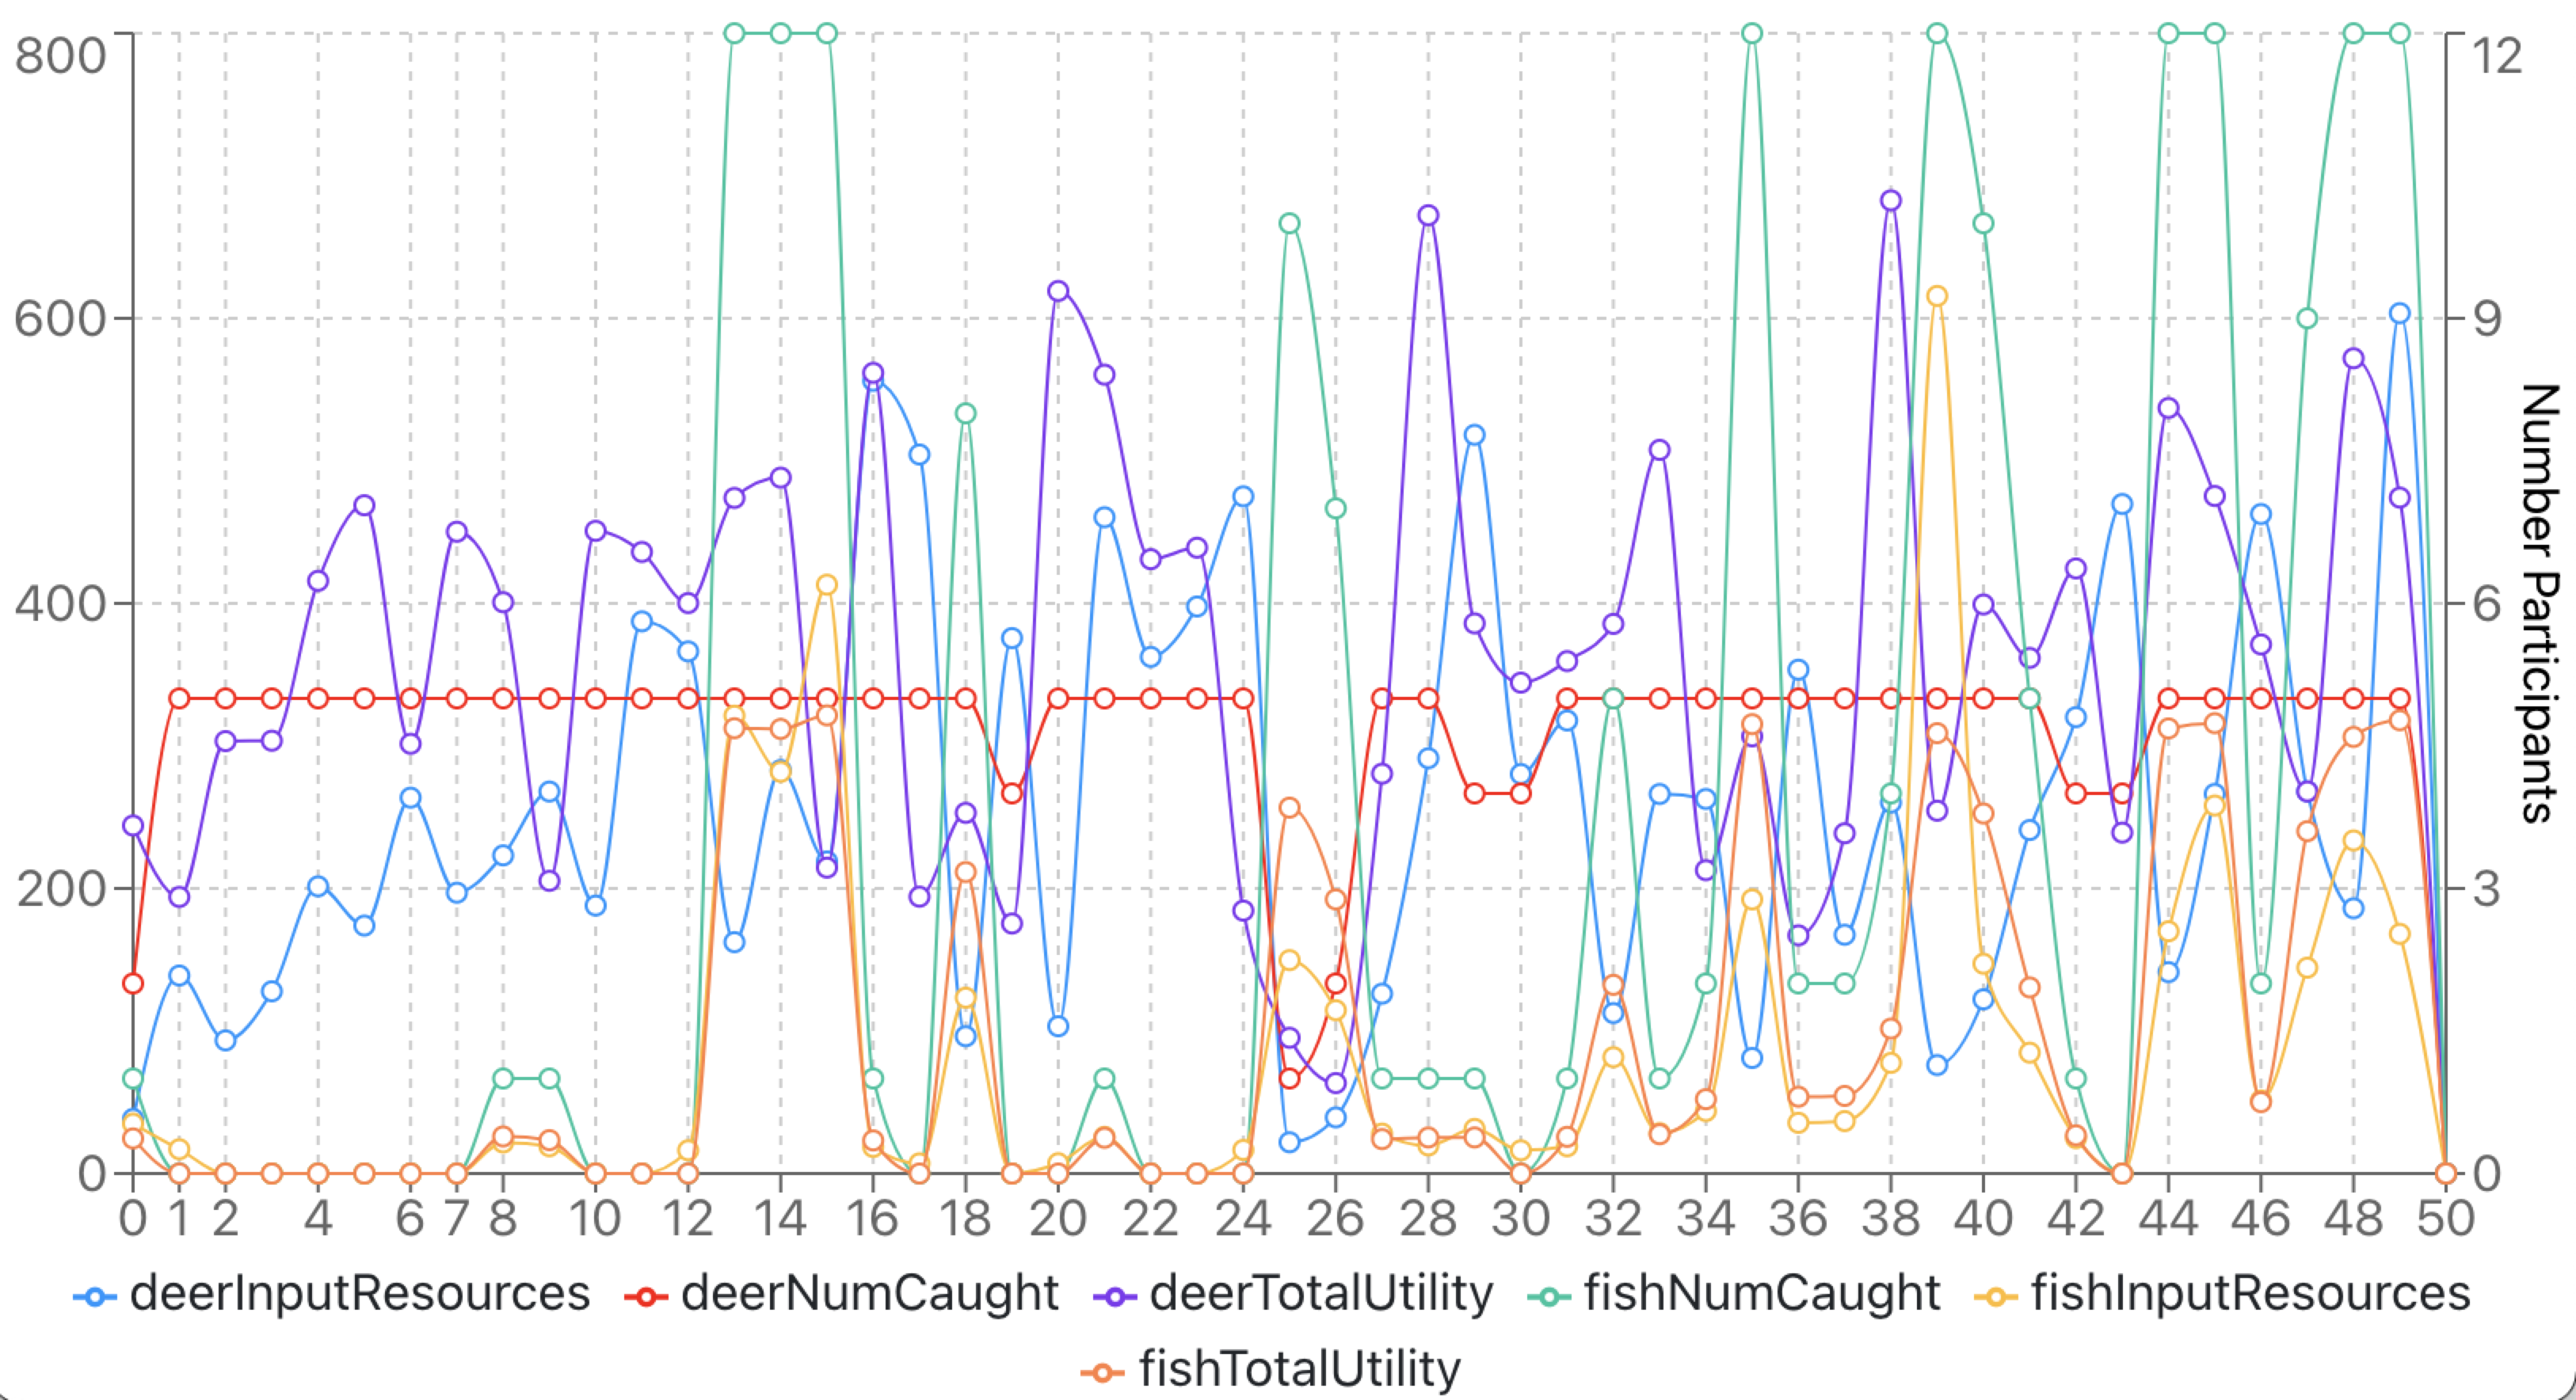
\includegraphics[width=0.8\textwidth]{14_team6_agentdesign/images/foraging.png}
    \caption{Foraging Visualisation}
    \label{fig:foraging}
\end{figure}

\subsection{Distribution of Roles} \label{subsec:Team6_Eval_Roles}

In this simulation result, we could see from Figure~\ref{fig:roles} that our agent is more active in government activities and spends more time managing government departments in the early stage. As time goes by, we are gaining less and less political power and Team 1 becomes the power house instead. This is basically consistent with what we expect to see in design level, because holding government roles could reduce our resources storage due to the cost of actions and will not be always beneficial to us. 

However, our voting strategy will not contribute that much to the election results, which is likely to be influenced by other islands' voting strategies and looks quite different from what we expected to see.
\begin{figure}[H]
    \centering
    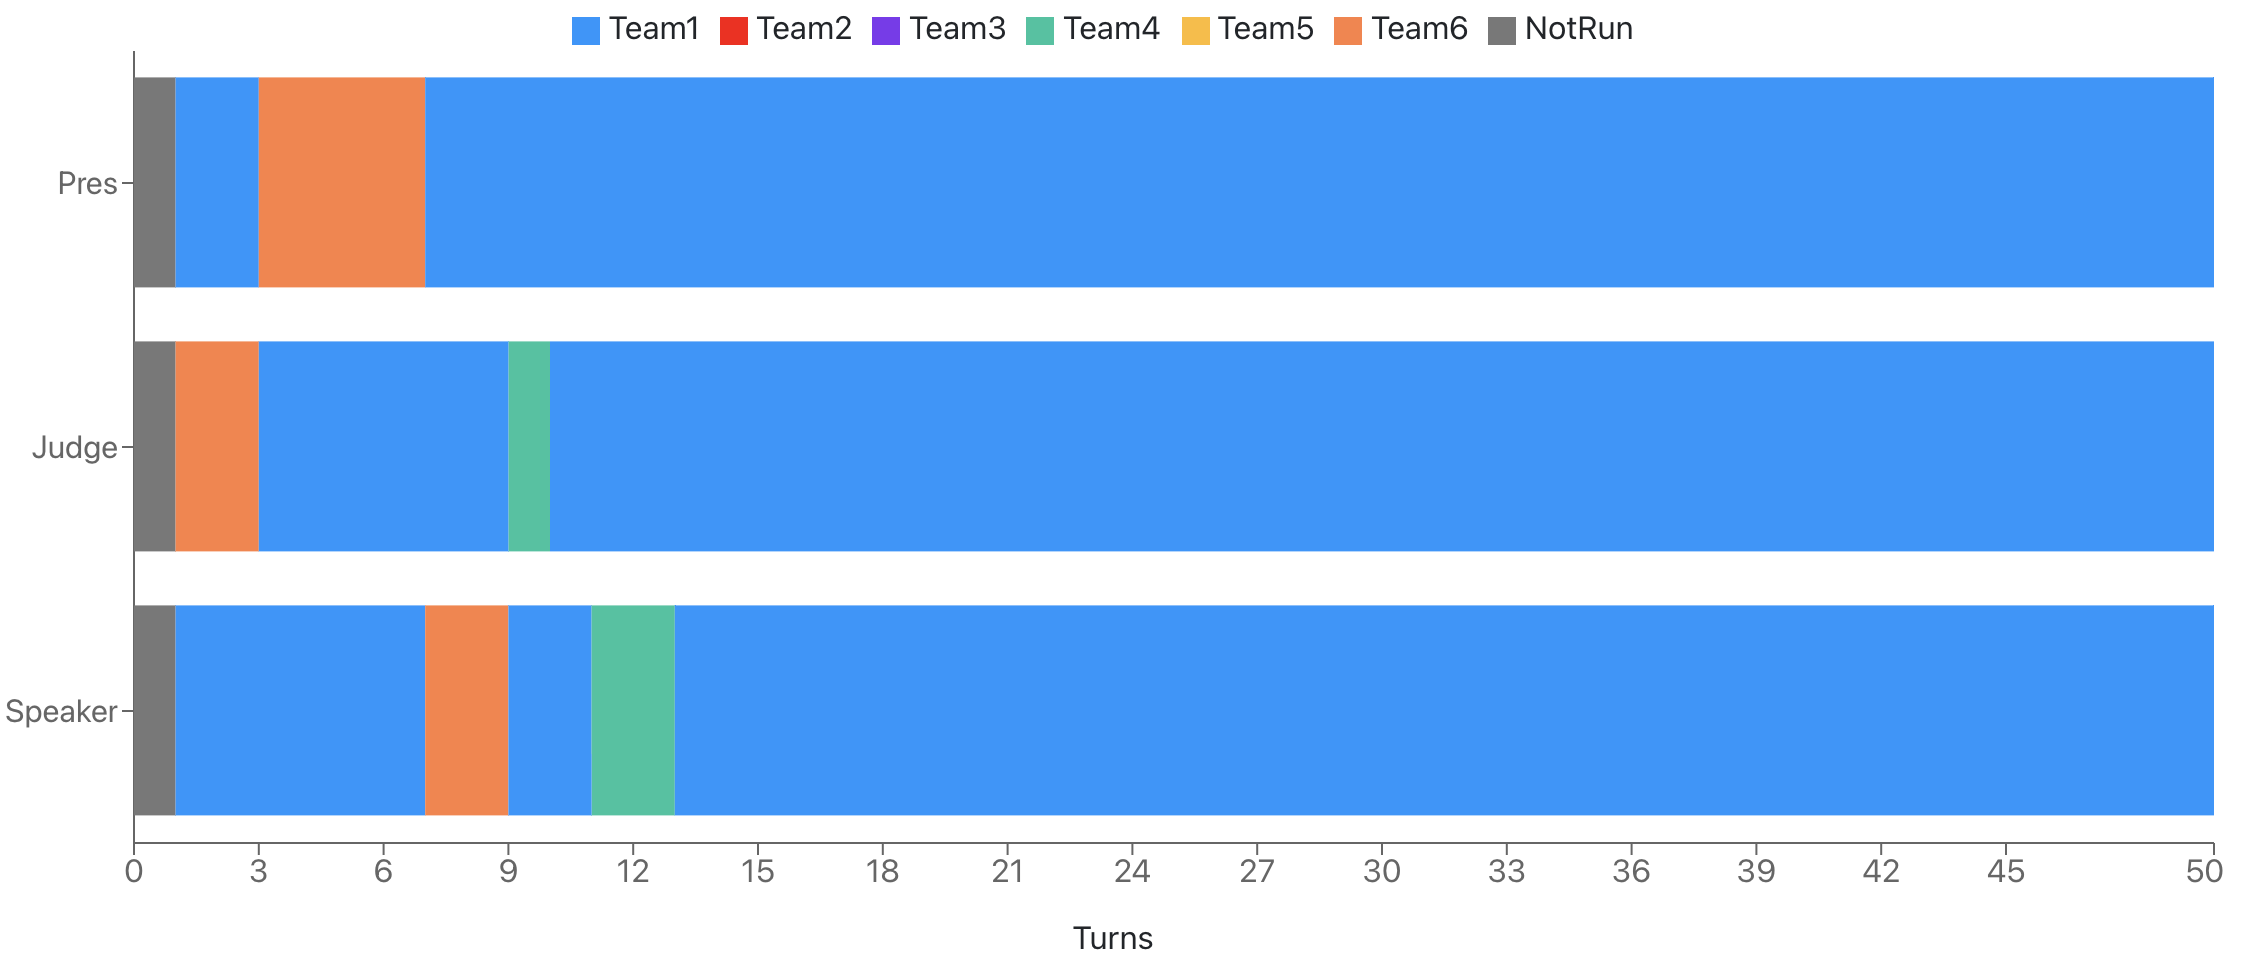
\includegraphics[width=0.8\textwidth]{14_team6_agentdesign/images/roles.png}
    \caption{Distribution of Roles}
    \label{fig:roles}
\end{figure}


\subsection{IIGO Payments} \label{subsec:Team6_Eval_IIGO}

In Figure~\ref{fig:IIGO}, compared to other islands, we manage to run with a lower expected tax level and actually paid more than that. Moreover, we never take more resources than allocated by President and never break the rule, which is also one of our advantages, as we don’t have to waste our resources in sanction payments for breaking rules. By doing this, we reduce the risk of common pool resource exhaustion in a short time, which contributes to the stability and sustainability for the whole system.\\
\begin{figure}[H]
    \centering
    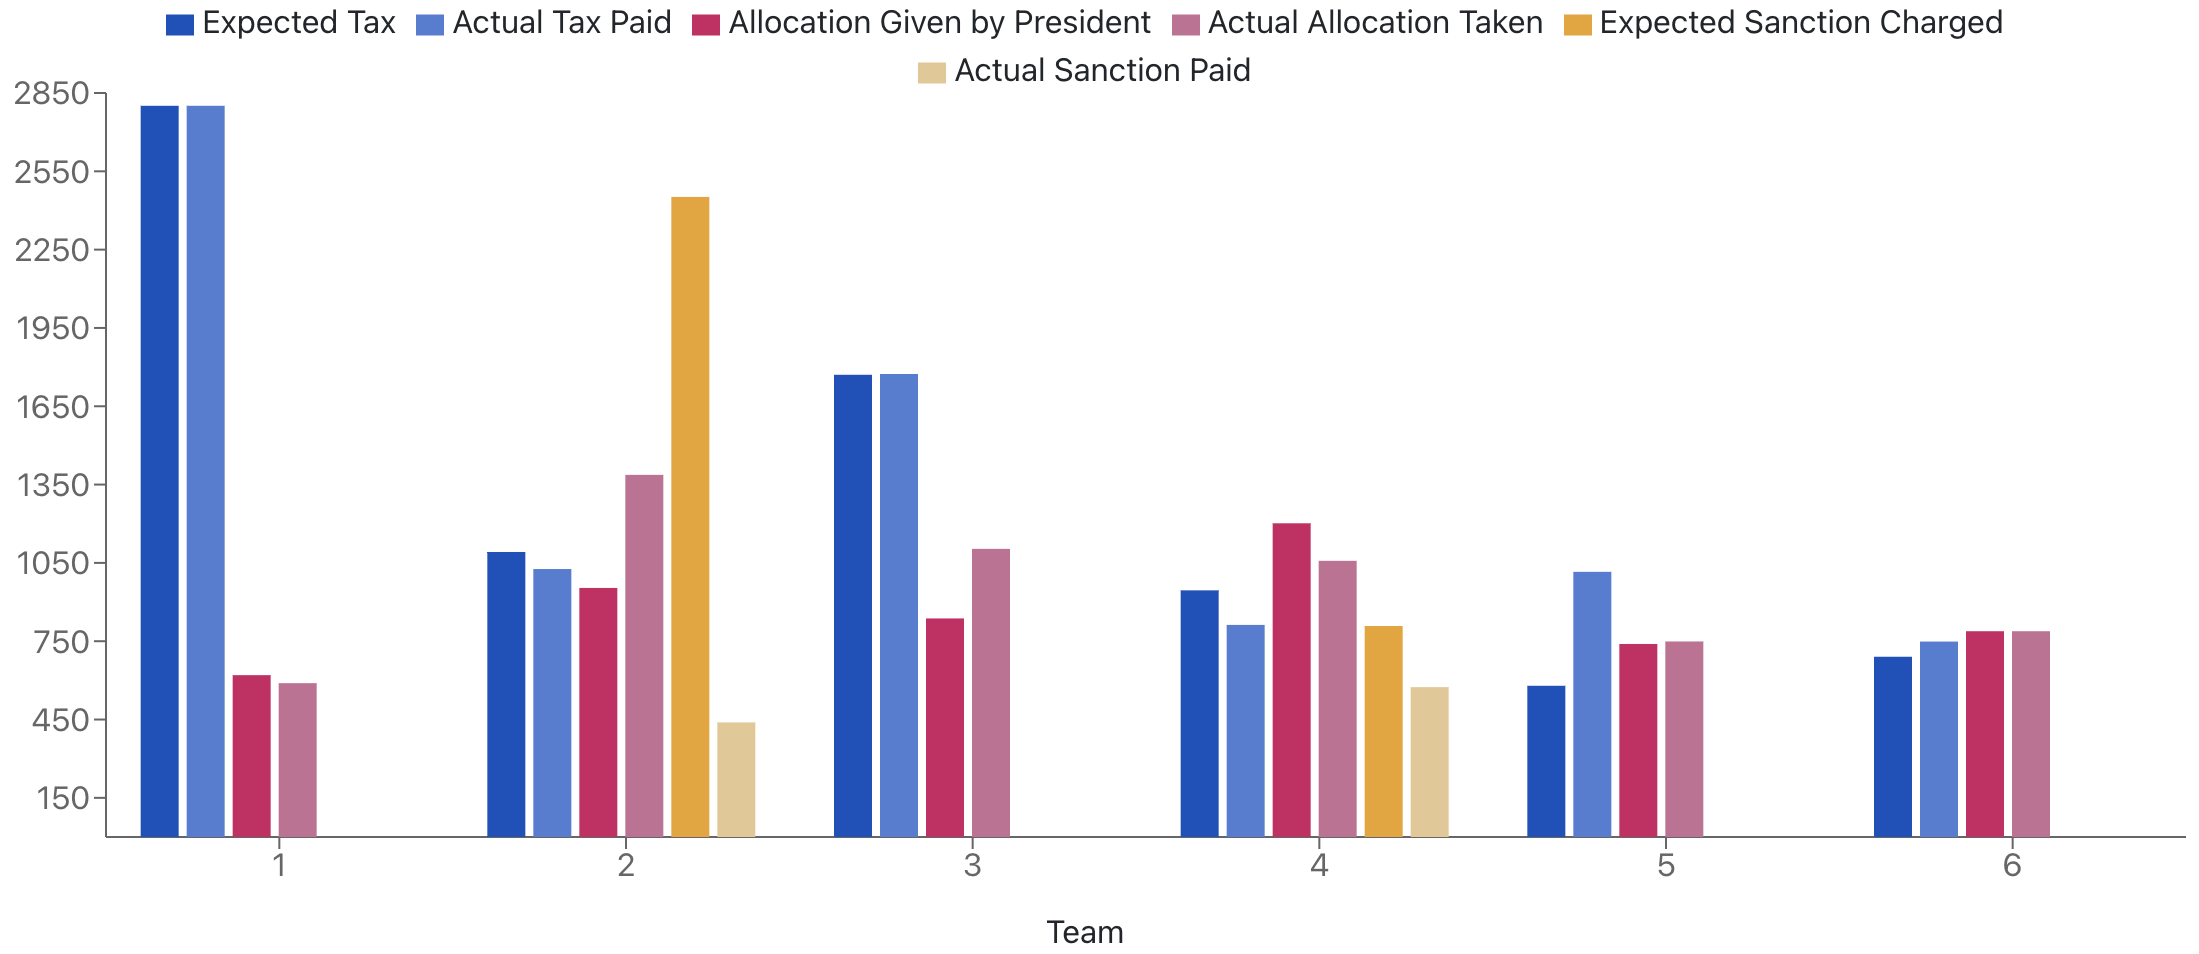
\includegraphics[width=0.8\textwidth]{14_team6_agentdesign/images/IIGO cost.png}
    \caption{IIGO Costs}
    \label{fig:IIGO}
\end{figure}

\subsection{IITO visualisation} \label{subsec:Team6_Eval_IITO}
The following plot shown in Figure~\ref{fig:IITO} visualises the transactions between islands in the IITO sessions. The size of a bubble represents the total magnitude of resources traded by each island. The width of each connecting edge between two islands represents the magnitude of transactions between the two islands. Islands that gave more resources than they receive are indicated by a red border, while islands that received more than they gave are indicated by a green border.

From the plot we could conclude that resources we have received are more than that given by us. Also, our bubble is the penultimate small one, which indicates that we are somewhat inclined to be self-isolated and lack of trade exchanges with other islands. This also could indicate that the friendship with other islands is somewhat not getting along really good based on our own opinion formation towards the other islands.
\begin{figure}[H]
    \centering
    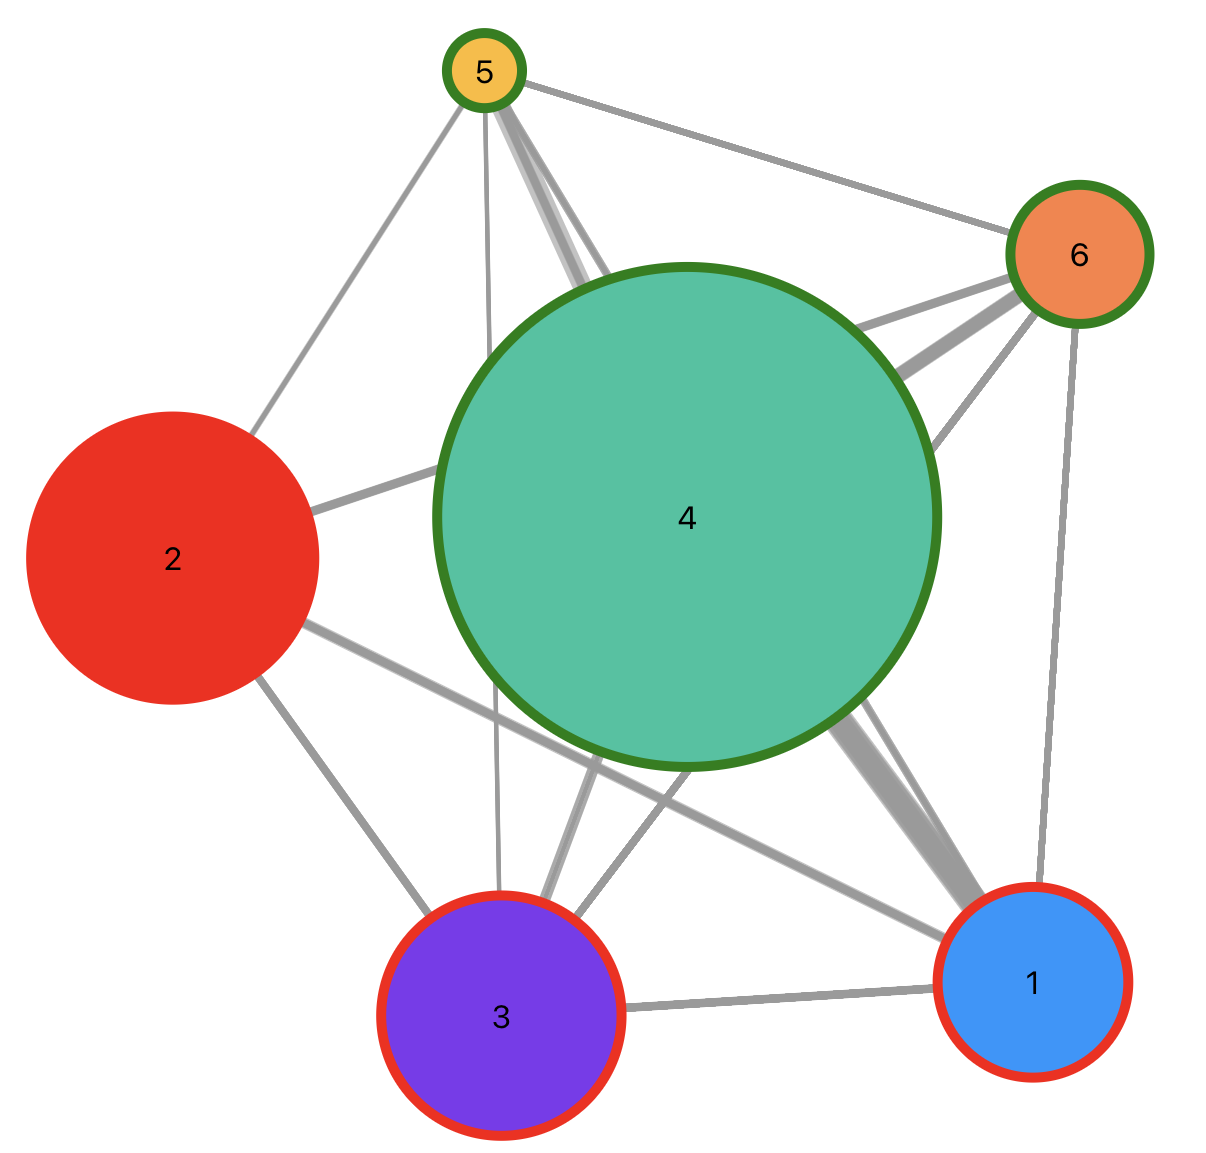
\includegraphics[width=0.4\textwidth, scale=0.1]{14_team6_agentdesign/images/IITO.png}
    \caption{IITO Visualisation}
    \label{fig:IITO}
\end{figure}

\subsection{Resources over time} \label{subsec:Team6_Eval_Resources}

Line charts listed in Figure~\ref{fig:all teams} show the changes about resources on each island and the common pool, as well as the sum of all resources over time. From the simulation results, we could conclude that every island manages to survive long enough, which indicates that our agent adapts well to the operation of the entire system and could automatically take advantage of situations in different specific situations. 

In addition, the resources change curve of our agent as seen in Figure~\ref{fig:team 6} is much smoother than that of some other agents, which shows that we actually have a good grasp of balancing out between income and expenditure of our resources. \\
\begin{figure}[H]
    \centering
    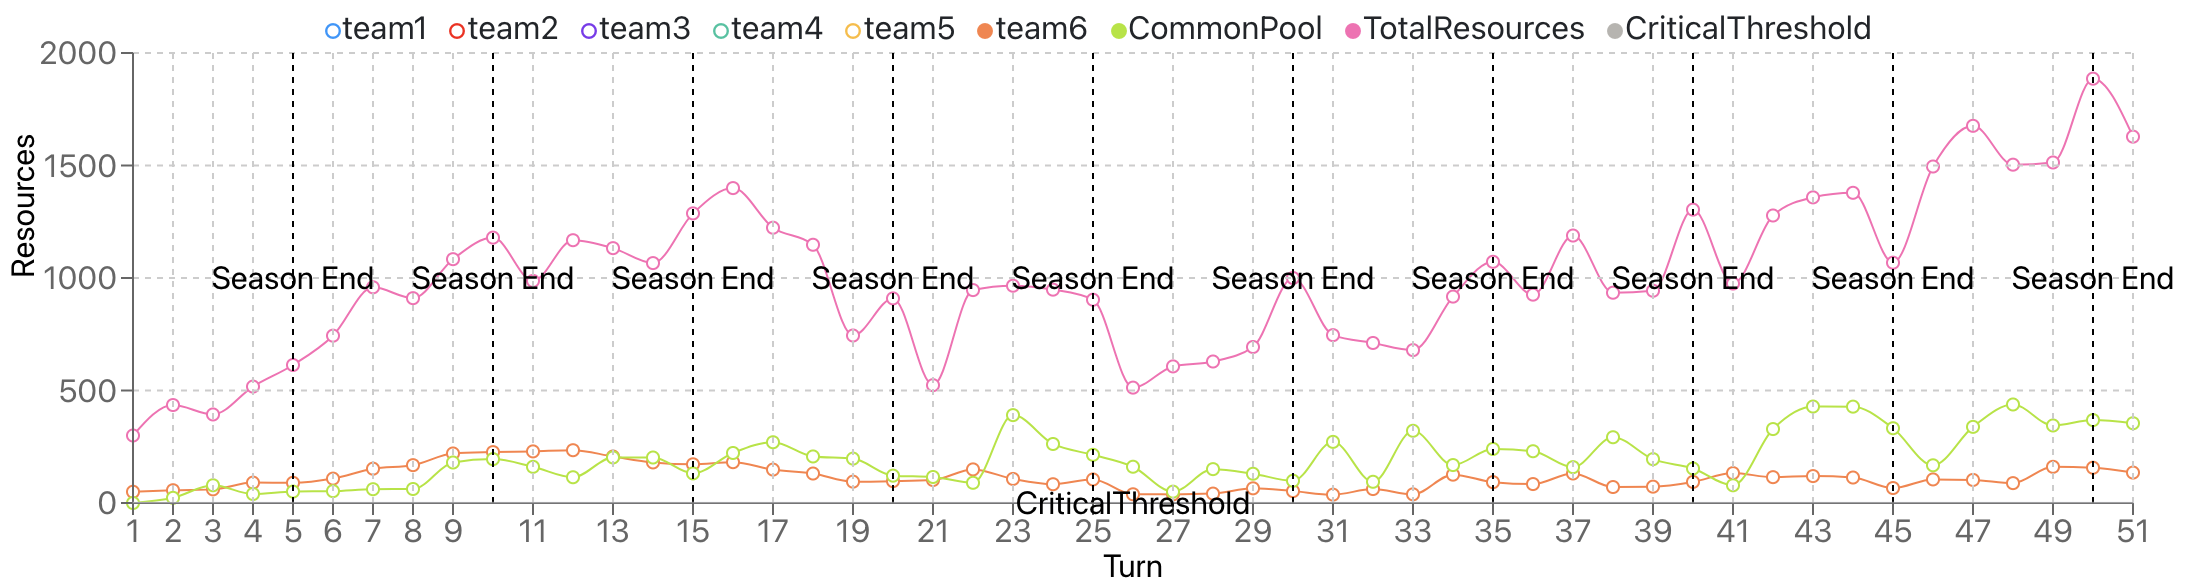
\includegraphics[width=0.8\textwidth]{14_team6_agentdesign/images/resources 1.png}
    \caption{Island 6 Resources Performance against CPR and Total Resources}
    \label{fig:team 6}
\end{figure}
\begin{figure}[H]
    \centering
    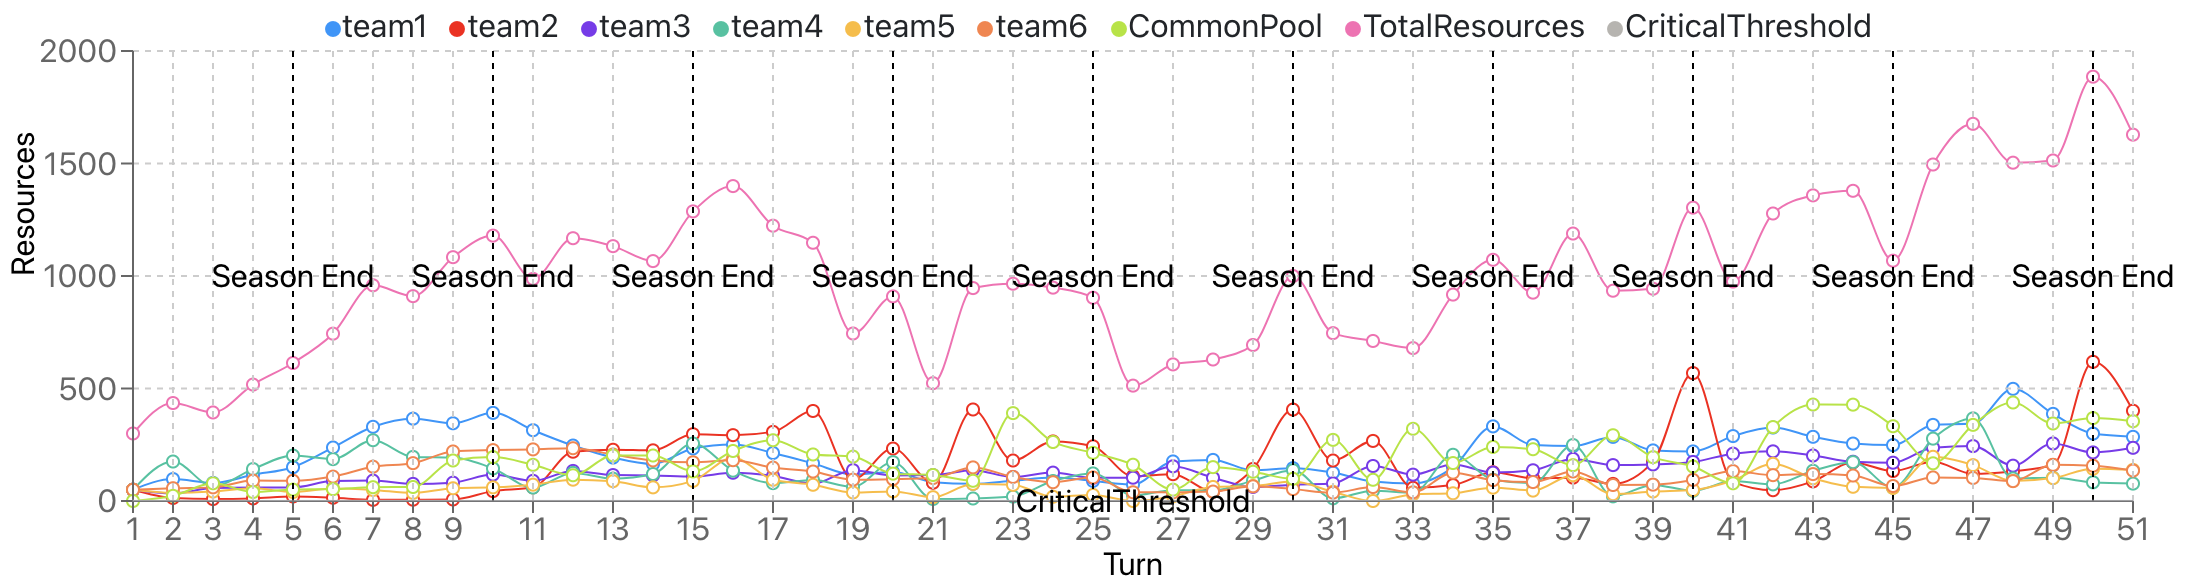
\includegraphics[width=0.8\textwidth]{14_team6_agentdesign/images/resources 2.png}
    \caption{Dynamic Resources Level of All Agents from Simulation}
    \label{fig:all teams}
\end{figure}

\section{Future Work} \label{sec:Team6_Future}
Our agent could hopefully be endowed with the ability of machine learning. By using reinforcement learning like Q-learning with CNN, it is possible to let the agent explore the environment by itself while generating the best decision based on what it has learned from the environment. It can become more optimised as the game goes on. However, some limitations became the main issue against the feasibility. To model the environment we need some libraries to build the environment framework. It turns out that programming language we use in this coursework did not supply sufficient machine learning libraries, which becomes a constraint to realise our idea. But we think the potential application of an agent with machine learning ability is feasible to build more robust strategies in dealing with the dilemmas on the overall game.